\documentclass[10pt,a4paper,printanswers]{upmc} 

\usepackage[T1]{fontenc}
\usepackage[utf8]{inputenc}
%\usepackage[english]{babel}
\usepackage{amsmath}
\usepackage{amssymb}
\usepackage[ruled,vlined,linesnumbered]{algorithm2e}
\usepackage{mathtools}
\usepackage[usenames,dvipsnames]{xcolor}
\usepackage{framed}
\usepackage[framemethod=tikz]{mdframed}
\usepackage{listings}    
\usepackage{subcaption}  
\usepackage{caption}   
\usepackage{pdfpages}

\global\mdfdefinestyle{graybox}{%
  linecolor=black,linewidth=1pt,%
 % leftmargin=1cm,rightmargin=1cm,%
  backgroundcolor=lightgray
}

\mdfdefinestyle{evaluation}{
    frametitlebackgroundcolor=black!15,
    frametitlerule=true,
    roundcorner=10pt,
    middlelinewidth=1pt,
    innermargin=0.5cm,
    outermargin=0.5cm,
    innerleftmargin=0.5cm,
    innerrightmargin=0.5cm,
    innertopmargin=\topskip,
    innerbottommargin=\topskip,
    frametitle={Evaluation}
}

%\printanswers
\framedsolutions
\renewcommand{\solutiontitle}{\noindent\textbf{Solution:}\par\noindent}

\usepackage[textwidth=18cm,textheight=25cm]{geometry}


\newcommand{\myline}{\noindent\makebox[\linewidth]{\rule{\textwidth}{0.7pt}}}
%\newcommand{\colonline}{: \hrulefill}
\newcommand{\mytilde}{\raise.17ex\hbox{$\scriptstyle\mathtt{\sim}$}}

\newcounter{mainmemorder}
\newcommand{\save}{\setcounter{mainmemorder}{\value{enumi}}}
\newcommand{\load}{\setcounter{enumi}{\value{mainmemorder}}}
\newcommand{\mytext}[1]{\colorbox{lightgray}{\texttt{#1}}}
\newcommand{\subsecline}{\texorpdfstring{\hrulefill}{}}

\newcommand{\Num}{Part 3}
\newcommand{\UE}{\scriptsize M1 ISI/SAR/IPS\\ ROS \& experimental robotics}

\newcommand{\Comment}[1]{\textcolor{red}{#1}}

\renewcommand*{\theenumi}{\#\thesubsection.\arabic{enumi}}
%\renewcommand*{\theenumii}{\theenumi.\arabic{enumii}}

\title{ROS and experimental robotics.\\ \Num: project.}



\lstset{language=matlab,
  basicstyle=\small\sffamily,
  keywordstyle=\color{dblue}\bfseries,  
  commentstyle=\color{dred}\textit,
  stringstyle=\color{dgreen}\ttfamily,
  extendedchars=true,
  frame=single, 
  numbers=left,
  backgroundcolor=\color{lgray}
}

\begin{document}

\maketitle

\section{Context, goal and evaluation of the project}
\vspace{-0.5cm}\myline\\
In this project, you will control a simulated and a real Turtlebot 3 burger mobile robot in a
realistic challenging environment, so as to make it navigate from one starting position to a goal
position with different tasks to solve on the path. The navigation should successively exploit:
\begin{itemize}
  \itemsep=-1pt
  \item images obtained from a simulated/real camera to detect and follow some lines,
  \item a laser scan obtained from a simulated/real LDS to detected and avoid some obstacles,
  \item and finally both of them to navigate in a challenging environment where both sensors are
        required together.
\end{itemize}
The project will take the form of 3 successive challenges relying on the sensorimotor capabilities
of the turtlebot, as illustrated in Figure~\ref{fig:challenges}.
%
\begin{figure}[!h]
  \centering
  \begin{subfigure}[b]{0.33\textwidth}
    \centering
    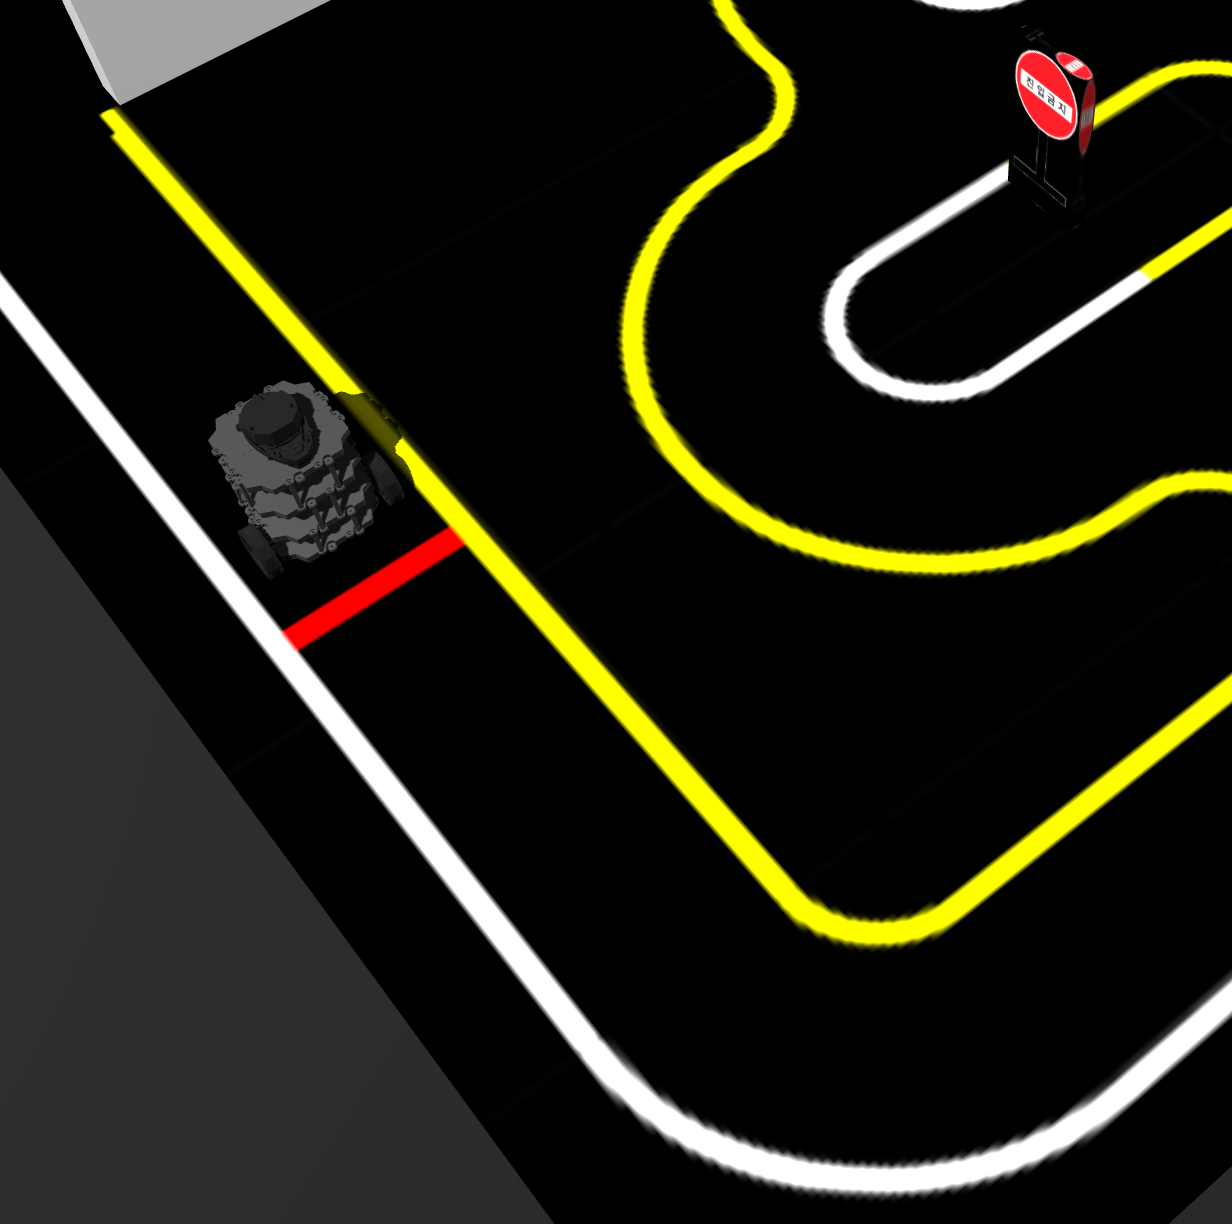
\includegraphics[width=5.5cm]{figures/illustr1_autorace.png}
    \caption{Challenge 1: line following}
    \label{fig:challenge1}
  \end{subfigure}
  %\hfill
  \begin{subfigure}[b]{0.33\textwidth}
    \centering
    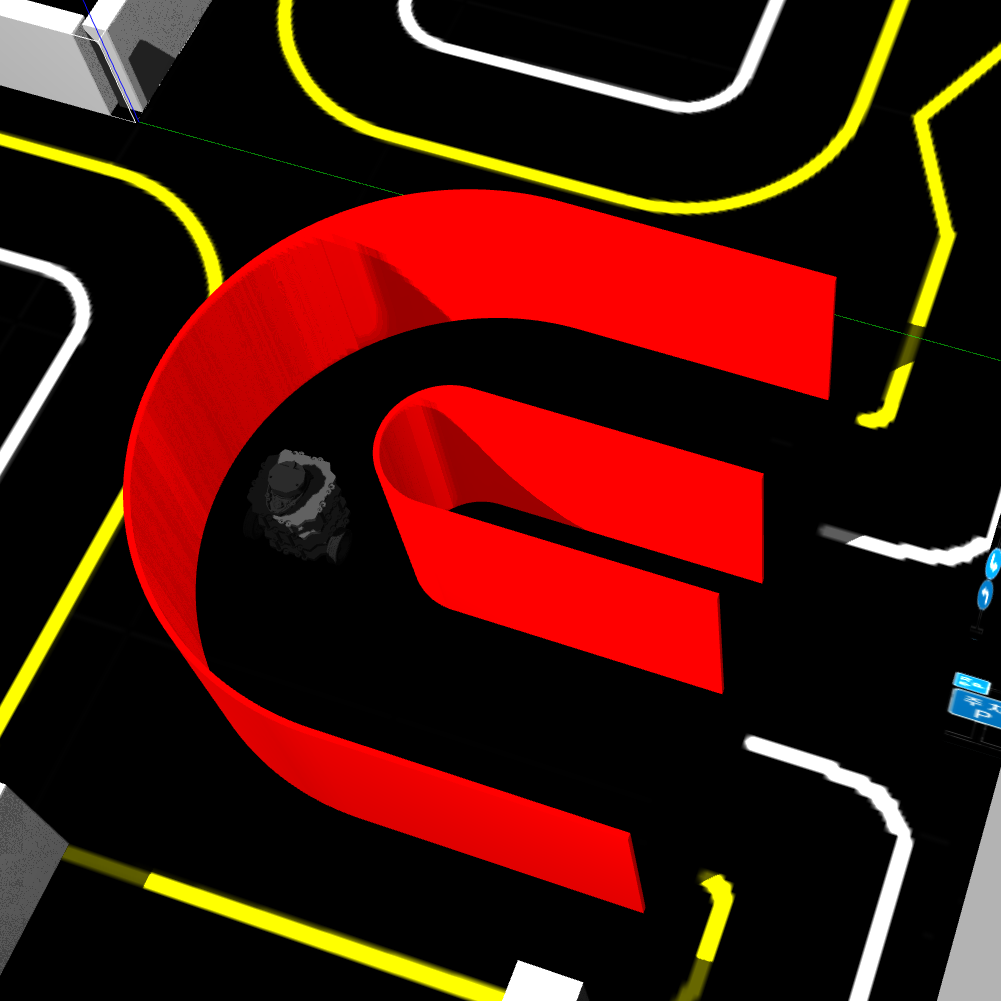
\includegraphics[width=5.5cm]{figures/illustr2_autorace.png}
    \caption{Challenge 2: corridor}
    \label{fig:challenge2}
  \end{subfigure}
  %\hfill
  \begin{subfigure}[b]{0.33\textwidth}
    \centering
    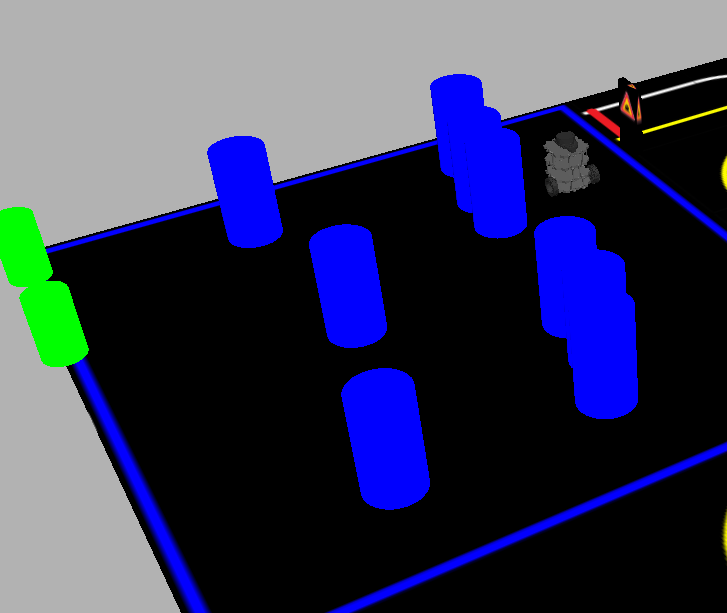
\includegraphics[width=5.5cm]{figures/illustr3_autorace_2.png}
    \caption{Challenge 3: cluttered environment}
    \label{fig:challenge3}
  \end{subfigure}
  \caption{Illustration of the gazebo world you will work on.}
  \label{fig:challenges}
\end{figure}

\subsection{Description of the organization of your work}

All your developments (code, launchfiles, scripts, gazebo worlds, configuration files, etc.) must be
placed inside one and unique ROS package named \texttt{projet}. You can find on Moodle the
corresponding package, including the simulated world we provide for the project (see
Figure~\ref{fig:gazebo_world}), together with the corresponding launchfile spawning a turtlebot 3
burger endowed with a LDS and camera sensors. Of course, these files only serve as a basis for your
requirements, and you are free to modify them accordingly\footnote{But please \textbf{do not modify}
  in any way the files in the different \mytext{turtlebot3} packages or worlds files.}. A
\mytext{rviz} config file allowing you do display the robot, the LDS data and the acquired image is
also provided.

\begin{enumerate}
  \item Unzip the package \texttt{projet} in your \texttt{catkin} workspace, launch
        \texttt{catkin\_make} and source the\\ \texttt{devel/setup.bash} file. If needed, use the
        \texttt{rospack profile} command to refresh your workspace.
  \item Use the provided launch file to launch \mytext{gazebo} and \mytext{rviz}. Test your
        teleoperation node written during part 1 so as to make the turtlebot move inside the
        provided environment, and check the consistency of the simulated sensors. \textbf{Please
          launch \mytext{rviz} and/or \mytext{gazebo} only when needed as it may require additional
          processing power. Also, do not hesitate to exploit \texttt{rosbag} to record and replay data
          from simulations (Gazebo) and/or the real robot.}
  \item On the basis on the provided launchfile, write a new launchfile dedicated to the real robot
        and allowing you tu visualize in \mytext{rviz} the sensors data.
\end{enumerate}

\noindent Congratulations, you are now ready to work on the project!

\subsection{Evaluation}

At the end of the project, you will have to:
\begin{itemize}
  \itemsep=-1pt
  \item send a compressed version of your \texttt{projet} package via Moodle;
  \item write a report on your work (more details below);
  \item make a demonstration of your work on the real robot during a competitive "race" against each
        other.
\end{itemize}

\subsubsection{Organization}
%
\begin{mdframed}[style=graybox]
  You are free to write as many nodes as you want, and organize your package at your will. The only
  mandatory requirement is that you write one/multiple launch file(s) allowing to launch everything
  required in simulation so as to assess your work.
\end{mdframed}
%
For the evaluation, your teachers will use this(ese) launchfile(s) to check if the tasks are
completed. Each launch file must launch all the required nodes (including \mytext{gazebo}),
set all the required arguments and parameters, so that no other commands have to be used to assess
your work.
But note that mastering all the tasks is not sufficient for you to reach the best grade. You must
also carefully comment all your code, whatever the language. In the end, the quality of your code
will be also evaluated, together with the fulfillment of traditional ROS \emph{good practices}
(like, not calling a service everytime a topic is changed, etc.).

\noindent Practically, we propose the following organization:
\begin{itemize}
  \itemsep=-1pt
  \item you can work by two, regardless of your initial group. No more than 1 group of 3 students
        per specialty (ISI, SMR, SAR) is allowed;
  \item you have now entire days of practicals (on Friday for ISI studients, on Monday for
        SAR/SMR students);
  \item for your organization, and because the real robot might not be alwayse available, use
        extensively \texttt{rosbag} to record and replay real data so as to design your algorithms.
\end{itemize}

Only one ROS package must then be uploaded to Moodle per student group. Do not forget to write down
your two names inside some kind of \texttt{README} file at the root of your package!
It is also important to understand that the "simulation" part of the project must be seen as a way to
test, evaluate, assess strategies that should then be implemented on the real robot. This transition
from simulation to reality is one of the key point in ROS architectures, and its versality should
help you in the process, providing you develop everything in a generic way (with parameters for
instance). Again, you can also benefit from recordings, \textbf{rosbag}, etc. to develop offline algorithms
that should work directly on the real robot, with real-time sensor data.
%
\begin{figure}[!h]
  \centering
  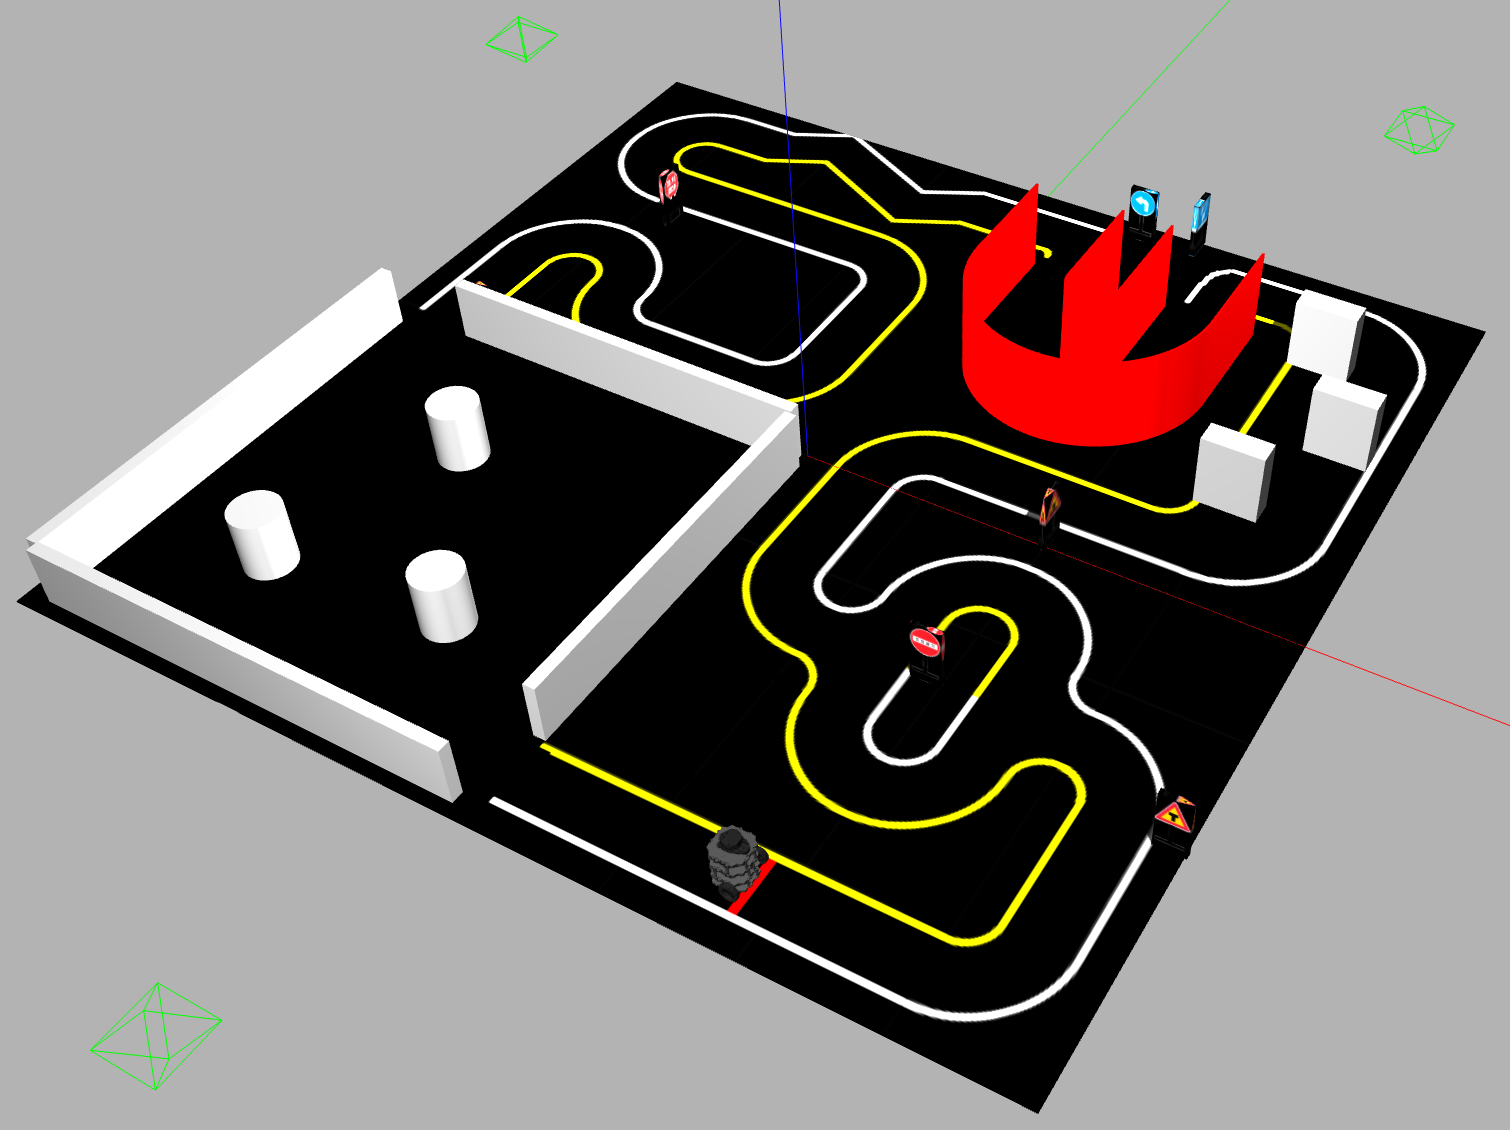
\includegraphics[width=12cm]{figures/world_autorace.png}
  \caption{The entire \mytext{gazebo} world, with the 3 three challenges to
    solve: (i) line following and obstacle avoidance, (ii) movement in a corridor, and (iii)
    navigation in a cluttered environment.}
  \label{fig:gazebo_world}
\end{figure}

\subsubsection{Report}
In addition to a zip/gz archive of your code, you also have to write a \LaTeX~report, with the
following requirements:
\begin{itemize}
  \itemsep=-1pt
  \item IEEE format, written in English;
  \item up to 3 pages, doubled-sided, 2 columns;
  \item with a mandatory organization given in the template available on Moodle.
\end{itemize}

Your document shall include detailed technical information regarding the ROS architecture of your
solution, including the list of the used nodes, the topics/messages they are using to communicate,
etc. In particular, you have to include a mandatory figure representing your architecture which must
be clearly explained in the text. The exact form/representation of this figure is up to you but must
be self-contained. The technical information should not only basically list the nodes you are using,
but also focus on the reason of your choices (which node, to do what, etc.) and justify the role of
each element in your architecture.

In addition to the previous explainations, it is also expected you provide a performance analysis of
your architecture in terms of e.g.\ speed, servoing errors statistics, precision, etc
(non-exhaustive list). To that end, you have to define, compute and analyze some features of your
choice and discuss the results you obtained.

A \LaTeX~template is available on Moodle. The resulting document is shown on
Page~\pageref{sec:report}.

\newpage
\section{Challenge 1: line following}
\vspace{-0.5cm}\myline\\

For this first challenge, you are supposed to code one or multiple nodes working together so that
the Turtlebot 3 follows some lines in the environment. But this challenge is not only about image
processing, since there will be also obstacles on the way to the second challenge.
%
You can also notice that two different line colors are used on the left and on the right sides of
the track, which sometimes split up when facing an intersection. This track following can also be
tested with the real robot: the robot must follow these lines made of a coloured tape stuck on the
floor (the exact color might be different from the one used in simulation), and detect if an
obstacle is present in front of it and navigate accordingly (this can involve an emergency stop
behavior).

In all this project, you must use the \texttt{OpenCv} library to process the image made available by
\mytext{gazebo} or the real robot on the corresponding ROS topic. You can find at the following
addresses some tutorials showing how to write Python code with \texttt{OpenCv}
\url{https://docs.opencv.org/master/d6/d00/tutorial_py_root.html}, see also the documentation in
\url{https://docs.opencv.org/4.2.0/pages.html}.\\

\noindent For this task, you will mainly have to:
\begin{itemize}
  \itemsep=-1pt
  \item build a new node which subscribes to the image topic published by \mytext{gazebo} or the
        real robot;
  \item interface ROS and OpenCV together; it requires a bridge to convert the image from the ROS
        \texttt{sensor\_msgs/Image} message to the correct OpenCV class. \texttt{CvBridge} provides
        the required functions to perform this conversion, see
          {\small{\url{https://wiki.ros.org/cv_bridge/Tutorials/ConvertingBetweenROSImagesAndOpenCVImagesPython}}}
  \item use basic \texttt{OpenCV} functions to process the image. Since you are trying to detect
        colored lines in the image, a simple binarization of the image, followed by an image moment
        computation (see \url{https://en.wikipedia.org/wiki/Image_moment}) might be an interesting
        step to extract some simple information you can use to drive the robot from the image, see
        Listing~\ref{lst:line_following} on page~\pageref{lst:line_following} ;
  \item finally, use this information to actually send a velocity command to the robot.
\end{itemize}

Some indications are provided in the following, guiding you on how to use \texttt{OpenCv} functions
in Python. You can also use visualization capabilities of \texttt{OpenCV} to display the current
image, the processed image, and the feature you are extracting from it (by displaying a text, a
point, etc.).

\newpage

\begin{mdframed}[style=evaluation]
  \textbf{Simulation:} for this task, you must write a launch file entitled
  \texttt{challenge1.launch} (i) spawning the robot at the beginning of the track with a correct
  orientation, and (ii) making the robot start its movement along the line, navigate among obstacles
  and eventyally stop accordingly if required (emergency stop).
\end{mdframed}

\section{Challenge 2: movement in a corridor}
\vspace{-0.5cm}\myline\\

For this second task, you have to code one or multiple nodes allowing the robot to navigate inside a
corridor, made of two adjacent walls guiding the robot from the first challenge (lines following) to
the third. It is clear here that the robot movement must be inferred mainly from the LDS data, with
a robot moving at the center of the corridor and following the left and right walls to the exit.
%
While this task can be solved in simulation, we also plan to build a small corridor for the real
robot. The objectives remain the same, and the robot must navigate safely between the two walls to
the exit.

\begin{mdframed}[style=evaluation]
  \textbf{Simulation:} for this task, you must write a launch file entitled
  \texttt{challenge2.launch} (i) spawning the robot at the beginning of the corridor with a
  correct orientation, and (ii) making the robot start its movement between the walls and stop
  at the exit.
\end{mdframed}

Note that if the simulation is oriented towards the validation of the navigation in the corridor
only, you will have to think about the succession of the two first challenges: first navigate on the
basis on visual data mostly, and then use the LDS to guide the robot between two walls. The way the
simulated and real robot will handled the succession of these two tasks is of particular importance
and must be dealt with correctly.

\section{Challenge 3: navigation in a cluttered environment}
\vspace{-0.5cm}\myline\\

In this third task, you have to code one or multiple nodes allowing the robot to navigate among
multiple obstacles placed randomly in the environment. Obviously, the robot must not touch any
obstacles during its movement and it must be driven towards the exit. The exit is materialized by two green posts placed randomly around the blue square delimiting the zone of this last challenge. 

In this task,
both sensors (LDS and camera) might be used to make the robot reach this target: the goal here is
then to make the robot reach the exit.

The same kind of objectives must be reach with the real Turtlebot 3 burger. A cluttered environment
will be used to assess the robot ability to navigate and reach the exit.

Again, the ability of your architecture to switch smoothly from the navigation in a corridor to a
navigation in a cluttered environment must be carefully addressed !

\begin{mdframed}[style=evaluation]
  \textbf{Simulation:} for this task, you must write a launch file entitled
  \texttt{challenge3.launch} (i) spawning the robot at the beginning of the cluttered environment
  with a correct orientation, and (ii) making the robot start its movement between the obstacles and
  stop when reaching the exit.
\end{mdframed}

\section{Conclusion: towards a competition between students on the real robot}
\vspace{-0.5cm}\myline\\

During the last week of the semester, we will organize a contest between students teams with the
real robot. Your robot will have to realize all the previous tasks, at once, as quick as possible.
Two tracks should be made available so as to face two teams with the same goal: reaching the
finish line. Basically, the winner will be declared on the basis on:
\begin{itemize}
  \item the time taken to reach the target, which should be as short as possible;
  \item the number of collision on the path to the target (obstacles, walls, etc.). In practice,
        each collision will produce some penalty to the team;
\end{itemize}

The exact conditions of the context will be communicated as soon as possible and will depend on the
conditions we will have in May.

\section{Appendix 1: technical datasheet of the Turtlebot 3 burger}
\vspace{-0.5cm}\myline\\

\begin{center}
  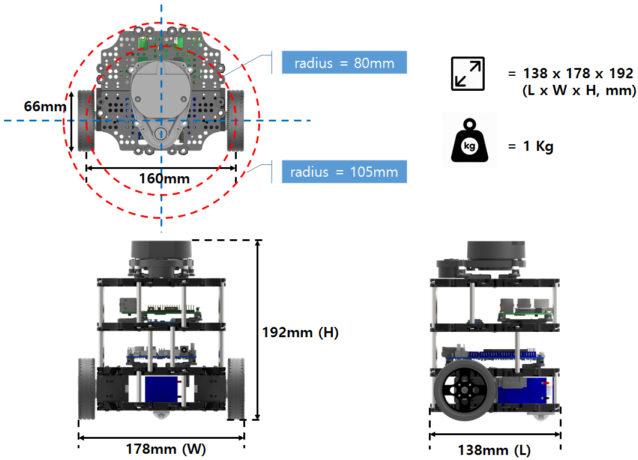
\includegraphics[width=13cm]{figures/turtlebot3_dimension1.png}\\
  \vspace{1cm}
  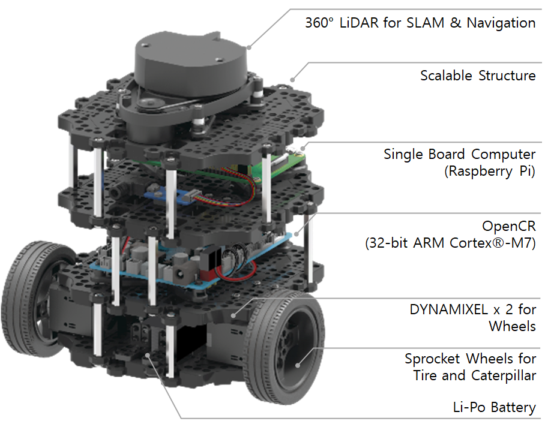
\includegraphics[width=13cm]{figures/turtlebot3_burger_components.png}
\end{center}

\newpage

\begin{center}
  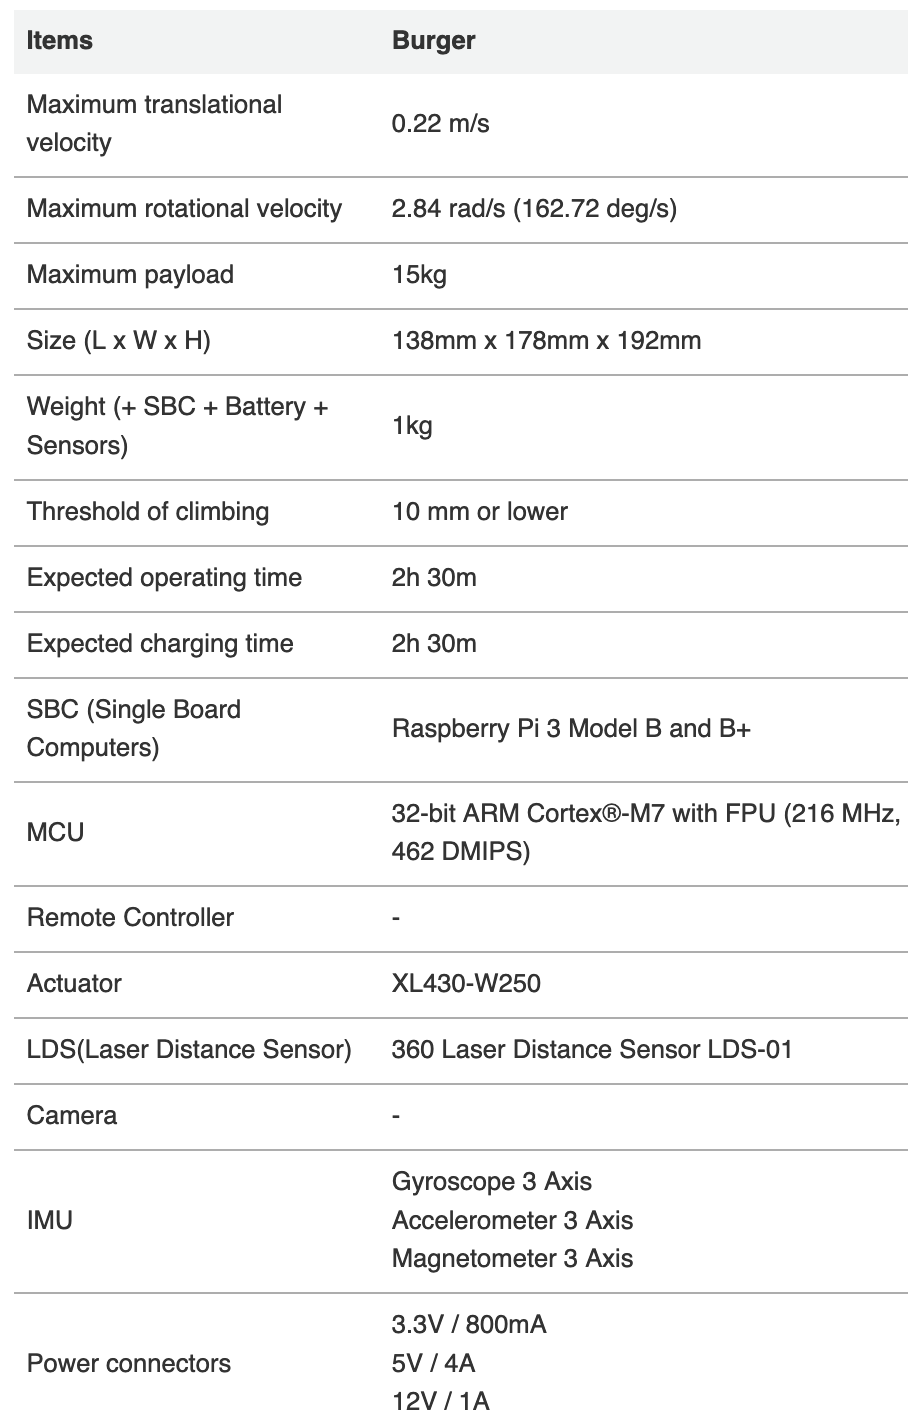
\includegraphics[width=8cm]{figures/datasheet1.png}\\
  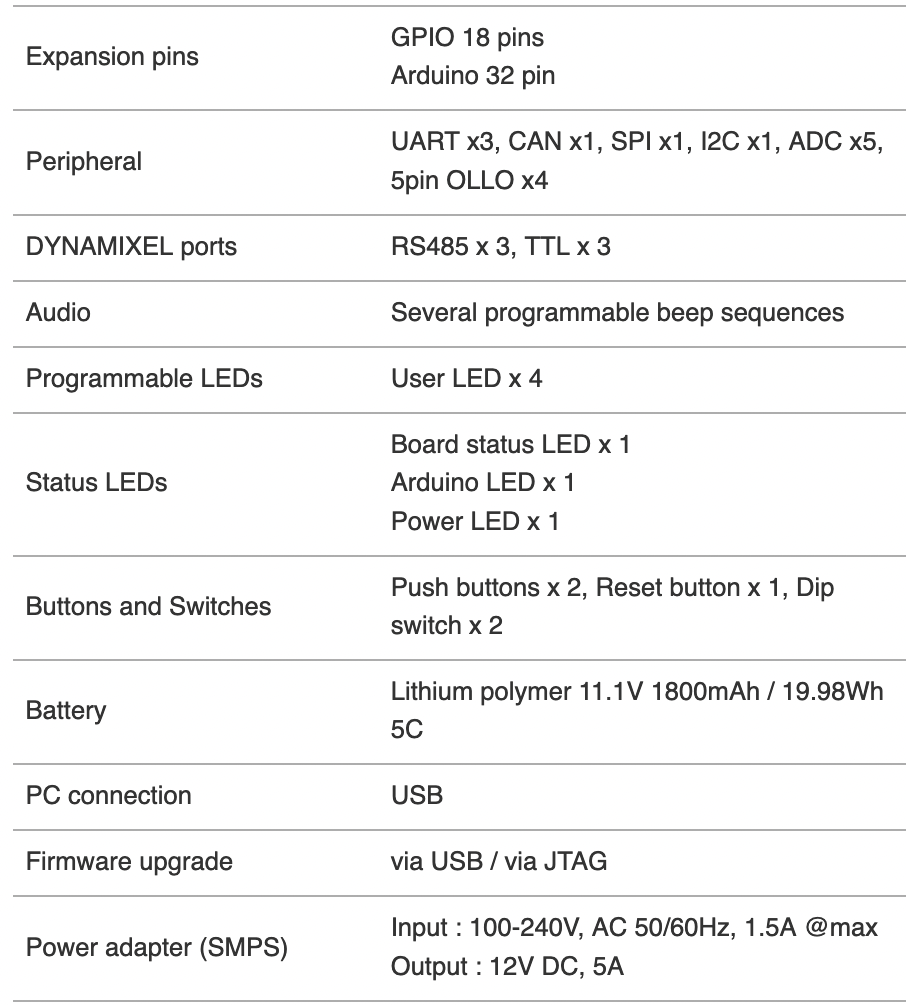
\includegraphics[width=8cm]{figures/datasheet2.png}
\end{center}


\newpage
\section{Appendix 2: starter code for \texttt{OpenCV}}
\lstinputlisting[
  caption=Code example for OpenCV, % Caption above the listing
  label=lst:line_following, % Label for referencing this listing
  language=Python, % Use Perl functions/syntax highlighting
  frame=single, % Frame around the code listing
  showstringspaces=false, % Don't put marks in string spaces
  numbers=left, % Line numbers on left
  numberstyle=\tiny, % Line numbers styling
  basicstyle=\footnotesize,
]{code/image_process.py}

\newpage
\section{Appendix 3: structure of the report}
\label{sec:report}
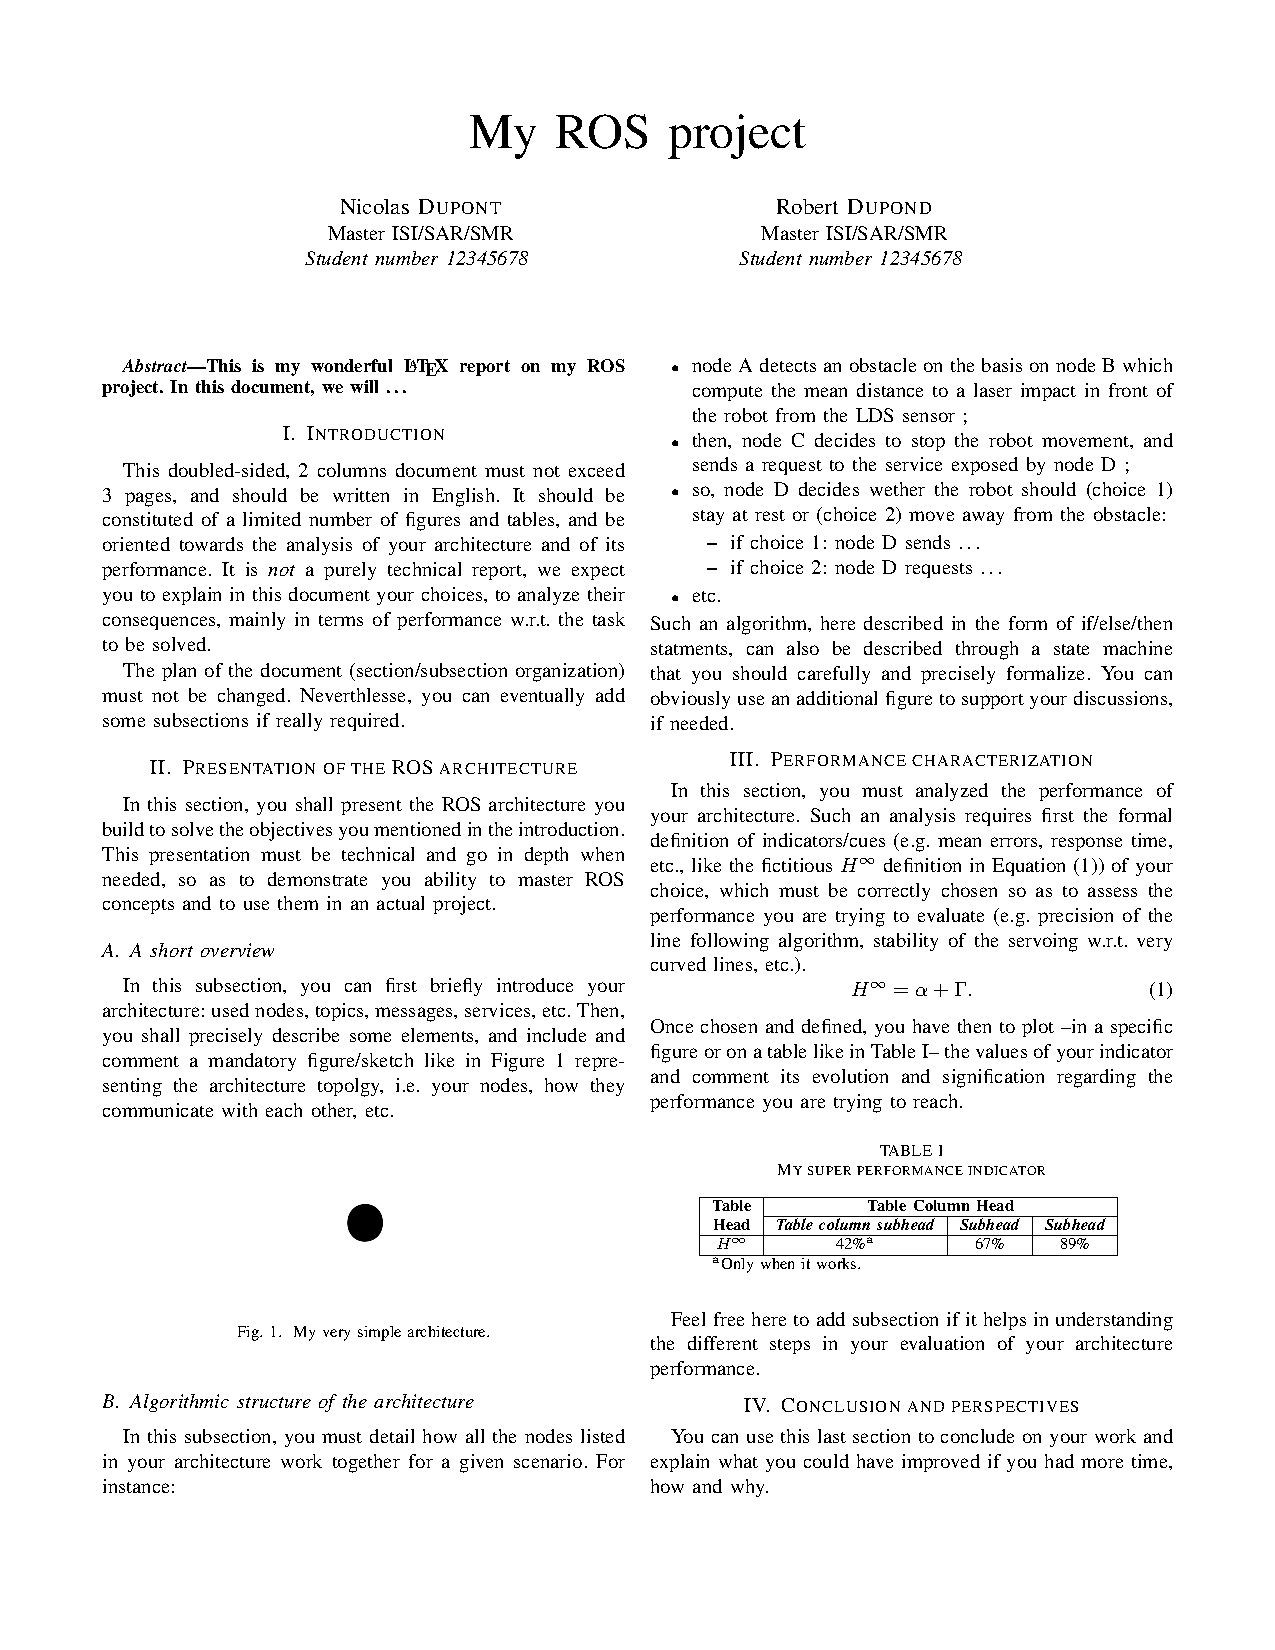
\includegraphics[width=\linewidth]{report/myproject.pdf}

\end{document}
